% !TEX root = ../report.tex
\subsection{Shared/Active repository} 

\begin{figure}[H]
\centering
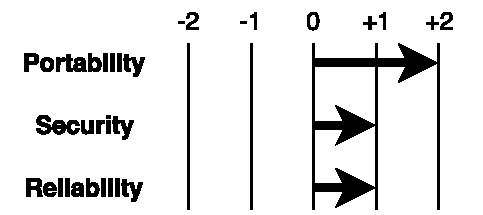
\includegraphics[scale=0.7]{6-evaluation/images/shared_active_repo_frm.pdf}
\caption{Force Resolution Map for Shared/Active Repository pattern.}
\label{fig:shared-active-repo-frm}
\end{figure}

According to Wikipedia, a reliable service is one that notifies the user if
delivery fails, while an ``unreliable'' one does not notify the user if delivery
fails. Based on this definition we can consider that the registry is reliable
because in case a push command doesn't work the user is notified (same system as
Github for example) by an error message/prompt and can try again.

Security is enhanced because the access to the registry is controlled by a login
and passwords for the users. Moreover, the push and pull commands in the
registry are also secure (see Brokered Authentication Pattern).

The docker registry is good for portability because whatever the environment of
the user everybody can subscribe and access this functionality.

The Shared Repository pattern has effects on other quality attributes such as
integrability, modifiability and re-usability. Figure \ref{fig:shared-active-repo-frm}
shows the FRM of Shared/Active Repository pattern.
